% ****** Start of file time_crystal_review.tex ******
%
%   Time Crystal: A Novel Phase of Matter of the 21st Century
%   Prepared with REVTeX 4.2 (APS template structure, apssamp.tex)
%
%   Required files in the same folder:
%     time_crystal_review.tex   (this file)
%     time_crystal_review.bib   (BibTeX database)
%     fig_kicked_ising.pdf      (Fig. 1)
%
%   Compile (BibTeX must be run):
%     1)  pdflatex time_crystal_review
%     2)  bibtex   time_crystal_review
%     3)  pdflatex time_crystal_review
%     4)  pdflatex time_crystal_review
%   or simply:  latexmk -pdf time_crystal_review
%
%   ---------------------------------------------------------------
%   PREPRINT  <->  REPRINT
%   The file is set up for PREPRINT (single column, wide spacing).
%   To get the two-column journal look later, change only the
%   class options below:  comment out "preprint," and uncomment
%   "reprint,".  Every display equation, the figure (figure*) and
%   the table (table*) are already sized for two-column output,
%   so nothing in the body needs to change.  Optionally uncomment
%   \raggedbottom further down while drafting in reprint mode.
%   ---------------------------------------------------------------
%
\documentclass[%
%preprint,
reprint,
superscriptaddress,
%groupedaddress,
%unsortedaddress,
%runinaddress,
%frontmatterverbose,
%preprintnumbers,
%nofootinbib,
%nobibnotes,
%bibnotes,
 amsmath,amssymb,
 aps,
%pra,
 prb,
%rmp,
 longbibliography,% print article titles in the reference list
 showkeys,% print \keywords{} under the abstract
 floatfix,
]{revtex4-2}
\usepackage{todonotes}
\usepackage{graphicx}% Include figure files
\usepackage{bm}% bold math
\usepackage{xcolor}
\usepackage[most]{tcolorbox}% pedagogical side boxes
\usepackage{microtype}
\usepackage[colorlinks=true,linkcolor=blue!50!black,citecolor=blue!50!black,
            urlcolor=blue!50!black]{hyperref}% add hypertext capabilities (load last)
%\usepackage[mathlines]{lineno}% Enable numbering of text and display math
%\linenumbers\relax % Commence numbering lines

% In reprint mode, \flushbottom can open large vertical gaps between
% paragraphs in a draft; uncomment for drafting, remove for submission.
%\raggedbottom

%--------------------------------------------------------------
% User macros and environments
%--------------------------------------------------------------
\newcommand{\Tr}{\operatorname{Tr}}
\newcommand{\ket}[1]{|#1\rangle}
\newcommand{\bra}[1]{\langle #1|}

% Pedagogical box; its width follows the current column, so it
% works unchanged in both preprint and reprint.
\newtcolorbox{pedbox}[1]{colback=gray!6,colframe=gray!55,boxrule=0.5pt,arc=1pt,
  left=6pt,right=6pt,top=4pt,bottom=4pt,fonttitle=\bfseries\small,title=#1,
  coltitle=black,colbacktitle=gray!18,before skip=8pt,after skip=8pt}

\begin{document}

%\preprint{Report number, if any}% top-right label; shown with "preprintnumbers"

\title{Time Crystals: A Novel Phase of Matter in the Twenty-First Century}
%\thanks{A footnote to the article title}%

% Replace the placeholder affiliations. Authors sharing an institution
% should use the identical \affiliation{} text: REVTeX merges them.
\author{Soumyabroto Majumder}
\affiliation{Department of Physics, The University of Burdwan, Burdwan 713104, India}

\author{Rahul Chandra}
\affiliation{Sankara Nethralaya Elite School of Optometry, DJ/16, Action Area 1D, New Town, Rajarhat, Kolkata 700156, India}

\author{Analabha Roy}
\affiliation{Department of Physics, The University of Burdwan, Burdwan 713104, India}

\author{Mahbub Rahaman}
 \email[Corresponding author: ]{mahbub.phys@gmail.com}
\affiliation{Harish Chandra Research Institute, A CI of Homi Bhabha National Institute,
Chhatnag Road, Jhunsi, Prayagraj, Uttar Pradesh 211019, India}

%\date{\today}% It is always \today, today, but any date may be explicitly specified

\begin{abstract}
Spontaneous symmetry breaking underlies the emergence of spatial order in condensed matter, occurring when a ground or thermal state has lower symmetry than its governing Hamiltonian. Wilczek proposed an analogous breaking of time translation symmetry, whereby a quantum system in its lowest-energy state would undergo persistent periodic motion. Although this equilibrium proposal was challenged, time crystalline order was subsequently formulated in nonequilibrium systems. In periodically driven systems, continuous time-translation symmetry reduces to a discrete symmetry, whose spontaneous breaking can produce a \emph{discrete time crystal} (DTC) with robust oscillations at an integer multiple of the drive period. Since generic driven systems absorb energy and heat toward infinite temperature, such order requires mechanisms including many body localization, prethermalization, or integrability to suppress heating. We review the Floquet algebraic origin of long lived oscillations and their dependence on driving protocols, initial states, and interactions, highlighting theoretical and experimental advances and the roles of symmetry, dimensionality, and dissipation in stabilizing DTCs.
\end{abstract}

\keywords{time crystals; Floquet systems; integrability; dynamical symmetries}
%Use showkeys class option if keyword display desired
\maketitle

%\tableofcontents% optional for a long review in preprint mode

%==============================================================
\section{\label{sec:intro}Introduction}
%==============================================================
The regular arrangement of atoms in space manifests 


Spontaneous symmetry breaking is a central organizing principle of condensed-matter physics. A ferromagnet breaks spin-rotation symmetry, while a crystal breaks continuous translational symmetry. In both cases, the ground state or thermal state exhibits less symmetry than the Hamiltonian from which it arises. In 2012, Wilczek asked whether \emph{time}-translation symmetry could be broken in the same way, such that a quantum system in its lowest-energy state would move periodically forever~\cite{Wilczek2012,ShapereWilczek2012}. The proposal was quickly challenged. Bruno~\cite{Bruno2013} and later Watanabe and Oshikawa~\cite{WatanabeOshikawa2015} showed that ground states and Gibbs states of local Hamiltonians cannot exhibit long-range order in time. Watanabe and Oshikawa defined this order using the correlator $\langle O(\mathbf{x},t)\,O(0,0)\rangle$, and later work made the result rigorous for Gibbs states~\cite{WatanabeOshikawaKoma2020}.

The idea was revived by moving away from equilibrium. In a periodically driven system, the Hamiltonian satisfies $H(t+T)=H(t)$, and only the \emph{discrete} time-translation symmetry $t\to t+T$ remains. A \emph{discrete time crystal} (DTC) breaks this symmetry: local observables respond with a period $mT$, where $m>1$ is an integer. The response must also be robust against perturbations and persist in the thermodynamic limit~\cite{Sacha2015,KhemaniPRL2016,ElseBauerNayak2016,vonKeyserlingk2016,YaoPRL2017}. Within a year of these proposals, signatures of period doubling were reported in trapped ions~\cite{Zhang2017} and in dense ensembles of nitrogen-vacancy (NV) centres~\cite{Choi2017}. Several reviews now cover the field broadly~\cite{SachaReview2018,SachaBook2020,KhemaniHistory2019,ElseAnnRev2020,ZaletelRMP2023}.

%==============================================================
\subsection{Floquet preliminaries}
For a $T$-periodic Hamiltonian, the evolution over one period is the Floquet operator
\begin{equation}
\begin{split}
U_F&=\mathcal{T}\exp\!\Big[-i\int_0^T H(t)\,dt\Big]\equiv e^{-iH_F T},\\
U_F\ket{\phi_\alpha}&=e^{-i\varepsilon_\alpha T}\ket{\phi_\alpha},
\end{split}
\end{equation}
where $\mathcal{T}$ denotes time ordering and we set $\hbar=1$. The quasienergies $\varepsilon_\alpha$ are defined only modulo $\Omega=2\pi/T$. Stroboscopic observables are $\langle O(nT)\rangle=\bra{\psi}U_F^{\dagger n}OU_F^n\ket{\psi}$. The discrete time-translation symmetry is simply the statement that $U_F$ is the same in every period.

\subsection{Defining discrete time-translation symmetry breaking}
A system is a discrete time crystal if, for a broad class of short-range-correlated initial states, there are local observables $O$ such that
\begin{equation}\label{eq:DTCdef}
\begin{gathered}
\lim_{n\to\infty}\;\lim_{L\to\infty}\;\langle O(nT)\rangle = f(nT),\\
f(t+mT)=f(t),\quad m>1,
\end{gathered}
\end{equation}
and if this behaviour is stable under small, generic perturbations of $U_F$~\cite{ElseBauerNayak2016,KhemaniPRL2016,vonKeyserlingk2016}. The order in which the limits are taken matters. In a finite system, period doubling eventually vanishes through tunnelling between symmetry-broken configurations on a timescale that grows with system size. An equivalent definition is given in terms of eigenstates. In a DTC with $m=2$, every Floquet eigenstate is a ``cat'' state, and the eigenstates form pairs whose quasienergies differ by exactly $\Omega/2$. This is called \emph{$\pi$-pairing}. Short-range-correlated initial states are superpositions of the two partners in each pair and therefore oscillate with period $2T$~\cite{ElseBauerNayak2016,vonKeyserlingk2016,KhemaniRepTheory2017}.

Throughout the chapter, we test each candidate system against four criteria:
\begin{itemize}\setlength\itemsep{1pt}
\item[(C1)] \textbf{Subharmonic response:} local observables oscillate with period $mT$, $m>1$.
\item[(C2)] \textbf{Rigidity:} the period remains locked at $mT$ over a finite range of drive parameters and does not drift continuously as they change.
\item[(C3)] \textbf{Persistence:} the oscillation lifetime diverges in the thermodynamic limit.
\item[(C4)] \textbf{Spatial long-range order}, so that the breaking of time-translation symmetry is collective rather than local.
\end{itemize}
Criterion (C2) distinguishes a time crystal from a driven harmonic oscillator, or from a single spin precessing in a field. Criterion (C4) distinguishes bulk order from an edge effect.

%==============================================================
\section{\label{sec:integrability}Integrability and the (usual) absence of oscillations}
%==============================================================
An integrable many-body system has an extensive set of local or quasi-local conserved charges $\{Q_k\}$ with $[H,Q_k]=[Q_k,Q_l]=0$~\cite{EsslerFagotti2016,IlievskiQuasilocal2016}. Free-fermion models such as the transverse-field Ising chain~\cite{LSM1961,Pfeuty1970} belong to this class, as do interacting Bethe-ansatz-solvable models such as the XXZ and Hubbard chains. Because these charges constrain the dynamics, integrable systems do not thermalize. After a quench they relax locally to a generalized Gibbs ensemble (GGE)~\cite{Rigol2007,VidmarRigol2016,Ilievski2015GGE}
\begin{equation}
\rho_{\rm GGE}=\frac{1}{Z}\exp\Big(-\sum_k\lambda_kQ_k\Big),
\end{equation}
where the Lagrange multipliers $\lambda_k$ are fixed by the initial values $\langle Q_k\rangle$. The quantum Newton's cradle~\cite{Kinoshita2006} demonstrates this memory of initial conditions. Periodically driven integrable systems similarly relax to a periodic GGE~\cite{LazaridesDasMoessner2014PRL}.

Note that integrable systems \emph{do} relax, just not to a thermal state. Expand the state in energy eigenstates, $\ket{\psi}=\sum_m c_m\ket{m}$. Then
\begin{equation}\label{eq:dephasing}
\begin{split}
\langle O(t)\rangle={}&\sum_m|c_m|^2O_{mm}\\
&+\sum_{m\neq n}c_m^*c_n\,O_{mn}\,e^{i(E_m-E_n)t}.
\end{split}
\end{equation}
In the thermodynamic limit, the energy differences $E_m-E_n$ form a continuum. The second term then dephases by the Riemann--Lebesgue lemma, leaving only the diagonal (GGE) part. Conservation laws determine \emph{where} the system relaxes, but they do not by themselves prevent relaxation. Persistent oscillations require more: the spectrum must contain an extensive set of exactly commensurate energy differences, and these differences must contribute finite weight to local observables. The next section explains what algebraic structure gives rise to such commensurability.

%==============================================================
\section{\label{sec:dynsym}Dynamical symmetries and persistent oscillations}
%==============================================================
\subsection{Definition}
An operator $A$ is a \emph{dynamical symmetry} with frequency $\omega$ if~\cite{Buca2019NatCommun,Medenjak2020PRB}
\begin{equation}\label{eq:dynsym}
[H,A]=\omega A .
\end{equation}
The Heisenberg equation $\dot A=i[H,A]=i\omega A$ then gives $A(t)=e^{i\omega t}A$ exactly, for every state. Equation~\eqref{eq:dynsym} also implies that $A$ is a ladder operator. If $H\ket{E}=E\ket{E}$, then $H(A\ket{E})=(E+\omega)A\ket{E}$. The spectrum therefore contains towers of levels spaced by exactly $\omega$, which is precisely the commensurability that Eq.~\eqref{eq:dephasing} requires. An ordinary conserved charge is the special case $\omega=0$.

\subsection{A generalized Mazur bound}
How much of a given observable $O$ is protected from dephasing? A clean answer comes from treating operators as vectors with the Hilbert--Schmidt inner product $(A|B)=\mathcal{D}^{-1}\Tr(A^\dagger B)$, where $\mathcal{D}$ is the Hilbert-space dimension. The Liouvillian superoperator $\mathcal{L}X=[H,X]$ is Hermitian with respect to this inner product, and $O(t)=e^{i\mathcal{L}t}O$. In a finite system, let $P_\lambda$ be the projector onto the eigenspace of $\mathcal{L}$ with eigenvalue $\lambda$. Then the infinite-temperature autocorrelation function is
\begin{equation}
C(t)=(O|O(t))=\sum_\lambda e^{i\lambda t}\,\|P_\lambda O\|^2 .
\end{equation}
Taking the time average of $e^{-i\omega t}C(t)$ isolates a single frequency:
\begin{equation}\label{eq:mazur}
\begin{split}
\lim_{\tau\to\infty}\frac{1}{\tau}\int_0^\tau dt\;e^{-i\omega t}\,C(t)&=\|P_\omega O\|^2\\
&\ge\sum_k\frac{|(A_k|O)|^2}{(A_k|A_k)} .
\end{split}
\end{equation}
Here $\{A_k\}$ denotes any set of mutually orthogonal dynamical symmetries with frequency $\omega$. The inequality holds because these operators span part of the eigenspace with eigenvalue $\omega$. For $\omega=0$, Eq.~\eqref{eq:mazur} reduces to the familiar Mazur--Suzuki bound on non-ergodicity~\cite{Mazur1969,Suzuki1971}. For $\omega\neq0$, it guarantees an oscillating component that never decays. In the thermodynamic limit, extensive observables $O=\sum_j o_j$ and (quasi-)local $A_k$ give overlaps proportional to $L$, so the bound per site remains finite~\cite{Medenjak2020PRB}.

The Floquet version follows by replacing $e^{i\mathcal{L}t}$ with the unitary superoperator $\mathcal{U}X=U_F^\dagger XU_F$. An operator obeying $\mathcal{U}A=e^{i\theta}A$ oscillates stroboscopically with phase $\theta$ per period. The case $\theta=\pi$ is special:
\begin{equation}\label{eq:pimode}
U_F^\dagger A\,U_F=-A\quad\Longleftrightarrow\quad\{U_F,A\}=0,
\end{equation}
which gives period doubling directly. Operators that satisfy Eq.~\eqref{eq:pimode} (at least approximately) and are localized in space are called \emph{$\pi$-modes}. They are central to Section~\ref{sec:kicked}.

\subsection{Examples}
\emph{Larmor precession.} In the isotropic Heisenberg chain in a field, $H=J\sum_j\mathbf{S}_j\cdot\mathbf{S}_{j+1}-h\sum_jS^z_j$, the total raising operator $S^+=\sum_jS^+_j$ satisfies $[H,S^+]=-hS^+$, so the magnetization precesses forever. This example satisfies (C1) and (C3) trivially, but it is not a time crystal. The frequency is set by the external field and is not locked (C2 fails), and the symmetry is broken explicitly rather than spontaneously.

\emph{$\eta$-pairing.} On a bipartite lattice, Yang's operator $\eta^\dagger=\sum_je^{i\boldsymbol{\pi}\cdot\mathbf{r}_j}c^\dagger_{j\uparrow}c^\dagger_{j\downarrow}$ obeys $[H_{\rm Hub},\eta^\dagger]=(U-2\mu)\eta^\dagger$ for the Hubbard model with chemical potential $\mu$~\cite{Yang1989}. The $\eta$-states have off-diagonal long-range order, so in this case a persistent oscillation \emph{coexists} with spatial long-range order (C4). Floquet extensions, in which the dynamical symmetry protects period-$mT$ responses in driven Hubbard models, were constructed in Ref.~\cite{ChinzeiIkeda2020}.

\emph{Interacting quasi-local dynamical symmetries.} The deepest example is the gapless XXZ chain in a magnetic field. Medenjak, Bu\v{c}a and Jaksch showed that this model has extensive quasi-local dynamical symmetries, inherited from the same quantum-group structure that produces its quasi-local conserved charges~\cite{IlievskiQuasilocal2016}. As a result, local observables oscillate indefinitely in the thermodynamic limit, with spatio-temporal long-range order~\cite{Medenjak2020PRB}. Related ``phantom'' spin-helix states, nearly exact eigenstates of XXZ magnets, have been observed to be long-lived in ultracold-atom experiments~\cite{Jepsen2022}.

\subsubsection*{Assessment against the criteria:}
Dynamical symmetries give exact, non-decaying oscillations (C1, C3), and in favourable cases long-range order (C4). Their frequency, however, is fixed by Hamiltonian parameters such as $h$ or $U-2\mu$. Generic perturbations destroy the symmetry, so (C2) fails. Dynamical symmetries explain \emph{why} oscillations can persist, but on their own they produce fine-tuned persistent oscillations rather than a phase. The Floquet setting changes this: a $\pi$-mode's frequency is pinned at $\Omega/2$ by the drive itself.

%==============================================================
\section{\label{sec:kicked}Worked example: the kicked Ising chain}
%==============================================================
\subsection{The model and the perfect-flip limit}
Consider an open chain of $L$ spins-$\tfrac12$. Each period consists of an Ising evolution followed by a transverse kick:
\begin{equation}\label{eq:UF}
\begin{split}
U_F&=\exp\Big(-i\sum_{j=1}^{L}g_j\sigma^x_j\Big)\\
&\quad\times\exp\Big(-i\sum_{j=1}^{L-1}J_j\sigma^z_j\sigma^z_{j+1}\Big),\\
g_j&=\tfrac{\pi}{2}(1-\epsilon_j),
\end{split}
\end{equation}
where we absorb the period into the dimensionless couplings. When $\epsilon_j=0$ the kick is a perfect spin flip: $e^{-i\frac{\pi}{2}\sigma^x}=-i\sigma^x$, so the kick equals $(-i)^LP$ with $P=\prod_j\sigma^x_j$, the global $\mathbb{Z}_2$ parity. Let $\ket{\mathbf{s}}$ be a $\sigma^z$ configuration with Ising energy $E_{\mathbf{s}}=\sum_jJ_js_js_{j+1}=E_{-\mathbf{s}}$. Because $P$ commutes with the Ising term, the cat states $\ket{\mathbf{s},\pm}=(\ket{\mathbf{s}}\pm\ket{-\mathbf{s}})/\sqrt2$ are exact Floquet eigenstates:
\begin{equation}
U_F\ket{\mathbf{s},\pm}=\pm(-i)^Le^{-iE_{\mathbf{s}}}\ket{\mathbf{s},\pm}.
\end{equation}
The spectrum is therefore exactly $\pi$-paired. A product state $\ket{\mathbf{s}}$ is an equal superposition of the two partners, so $\langle\sigma^z_j(nT)\rangle=(-1)^ns_j$, which is period doubling.

The real question is what happens when $\epsilon\neq0$. For non-interacting spins ($J_j=0$), each spin simply rotates by $\pi(1-\epsilon)$ per period, so $\langle\sigma^z(nT)\rangle=\cos[n\pi(1-\epsilon)]$. The response is a beat whose frequency drifts with $\epsilon$, and (C2) fails. Interactions are what lock the period.

\subsubsection*{Toggling frame: period doubling as ferromagnetism}
If kick is $e^{-i g\sum\sigma^x}=(-i)^LP\,e^{i\frac{\pi\epsilon}{2}\sum_j\sigma^x_j}$, since; $P$ commutes with everything else and $P^2=1$,
\[
U_F^2=(-1)^L\Big[e^{i\frac{\pi\epsilon}{2}\sum_j\sigma^x_j}\,e^{-i\sum_jJ\sigma^z_j\sigma^z_{j+1}}\Big]^2 .
\]
Over two periods, the system evolves under a Floquet transverse-field Ising model with a small field $\pi\epsilon/2$. Period doubling in the lab frame is ferromagnetic (or spin-glass) order in this toggling frame. The order survives as long as the field is weaker than the coupling, $\pi\epsilon/2<J$, anticipating the exact result below. It also shows why the clean bulk must eventually fail at finite energy density: as in the Landau--Peierls argument, there is no finite-temperature order in one dimension.

\subsection{Jordan--Wigner solution}
Introduce Majorana operators $\gamma_{2j-1}=\big(\prod_{k<j}\sigma^x_k\big)\sigma^z_j$ and $\gamma_{2j}=\big(\prod_{k<j}\sigma^x_k\big)\sigma^y_j$, which obey $\{\gamma_a,\gamma_b\}=2\delta_{ab}$~\cite{LSM1961,Kitaev2001}. Both terms in Eq.~\eqref{eq:UF} are quadratic:
\begin{equation}
\sigma^x_j=i\gamma_{2j-1}\gamma_{2j},\qquad \sigma^z_j\sigma^z_{j+1}=i\gamma_{2j}\gamma_{2j+1}.
\end{equation}
A quadratic generator $H=\frac{i}{4}\sum_{ab}\mathcal{A}_{ab}\gamma_a\gamma_b$, with $\mathcal{A}$ real and antisymmetric, acts linearly on the Majoranas: $e^{iH}\gamma_ae^{-iH}=\sum_b(e^{\mathcal{A}})_{ab}\gamma_b$. Hence
\begin{equation}\label{eq:R}
\begin{gathered}
U_F^\dagger\gamma_aU_F=\sum_bR_{ab}\gamma_b,\\
R=e^{\mathcal{A}_K}e^{\mathcal{A}_I}\in SO(2L),
\end{gathered}
\end{equation}
where $(\mathcal{A}_K)_{2j-1,2j}=2g_j$ and $(\mathcal{A}_I)_{2j,2j+1}=2J_j$. All many-body dynamics thus reduces to powers of a $2L\times2L$ orthogonal matrix. The eigenvalues $e^{\pm i\theta_k}$ of $R$ define the single-particle quasienergies $\theta_k$, and a Majorana mode with $\theta=\pi$ is a $\pi$-mode in the sense of Eq.~\eqref{eq:pimode}.

Note that $\gamma_1=\sigma^z_1$ does not appear in the Ising term. At $\epsilon=0$ the kick maps $\gamma_1\to-\gamma_1$, so $\sigma^z_1$ is an \emph{exact} $\pi$-mode. For $\epsilon\neq0$, $\gamma_1$ mixes into the bulk, but a dressed $\pi$-Majorana $\Psi_\pi=\sum_av_a\gamma_a$, localized exponentially near the edge, survives. For uniform couplings this happens whenever $\pi/2-g<J$ (with $J<\pi/4$)~\cite{Thakurathi2013,KhemaniPRL2016}, which matches the toggling-frame estimate exactly. For $J=\pi/8$ the condition reads $\epsilon<\epsilon_c=2J/\pi=1/4$. Figure~\ref{fig:KI}(a) shows the corresponding modes pinned at $\theta=\pi$, separated from the bulk band, which reaches $\pi$ and closes the gap at $\epsilon_c$. In a finite chain the two edge modes hybridize, and the splitting $\propto e^{-L/\xi}$ sets the time at which a finite system loses period doubling.

% Fig. 1 placed right after its first citation (APS convention).
\begin{figure*}[t]
\todo[inline]{If possible, drop figures and relevant descriptions in the corresponding sections}
\centering
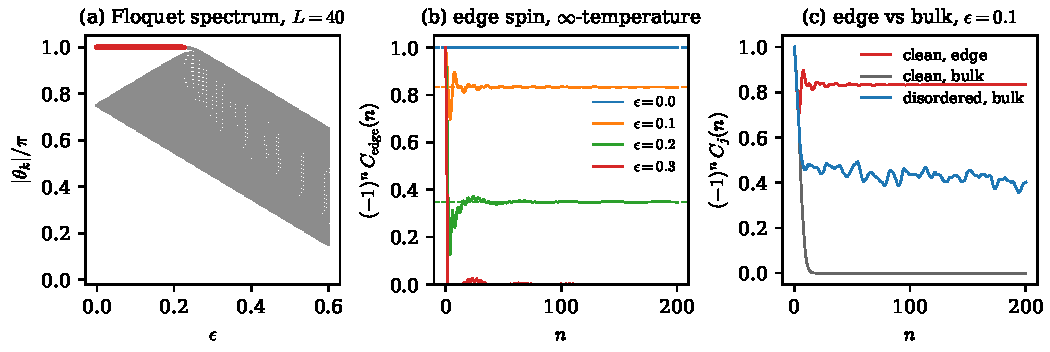
\includegraphics[width=\textwidth]{figs/fig_kicked_ising.pdf}
\caption{Kicked Ising chain, Eq.~\eqref{eq:UF}, with $J=\pi/8$ (so that $\epsilon_c=1/4$). (a) Single-particle quasienergies $|\theta_k|$ of the clean chain ($L=40$) versus kick imperfection $\epsilon$. Red points mark the edge $\pi$-Majoranas pinned at $\theta=\pi$. (b) Infinite-temperature edge autocorrelation $(-1)^nC_{\rm edge}(n)=(-1)^n(R^n)_{11}$ for a clean chain of $L=150$. Dashed lines show the bound of Eq.~\eqref{eq:mazur}, $\sum|v_1|^2$ over the $\pi$-eigenspace, which is saturated. (c) Edge ($j=1$) and bulk ($j=40$) spins for $L=80$, $\epsilon=0.1$, from Eq.~\eqref{eq:det} (verified against exact diagonalization). The clean bulk signal decays within a few periods. With disorder ($J_j\in J[0.5,1.5]$, $g_j\in\frac{\pi}{2}(1-\epsilon)+[-0.15,0.15]$, uniform, 40 realizations) it persists.}
\label{fig:KI}
\end{figure*}

\subsection{Edge spin: the bound is saturated}
The infinite-temperature autocorrelation of the edge spin follows from Eq.~\eqref{eq:R} and $(\gamma_a|\gamma_b)=\delta_{ab}$:
\begin{equation}
C_{\rm edge}(n)=(\sigma^z_1|\sigma^z_1(nT))=(R^n)_{11}.
\end{equation}
Within the linear Majorana sector, Eq.~\eqref{eq:mazur} holds with \emph{equality}:
\begin{equation}
\overline{(-1)^nC_{\rm edge}(n)} =\big\|P_\pi\,\gamma_1\big\|^2 =\sum_{v\in\ker(R+1)}|v_1|^2 .
\end{equation}
Here, the overline denotes a time average and the sum runs over an orthonormal basis of the $\pi$-eigenspace of $R$. Figure~\ref{fig:KI}(b) confirms this numerically. For every $\epsilon<\epsilon_c$ the stroboscopic edge signal approaches the dashed line given by the $\pi$-mode weight. Its frequency stays locked at $\Omega/2$ while its amplitude decreases continuously, and it vanishes for $\epsilon>\epsilon_c$. This is the Floquet analogue of a \emph{strong zero mode}~\cite{Fendley2016,AliceaFendley2016,Kemp2017}. It is an operator statement that holds for the entire spectrum, which is why period doubling appears even at infinite temperature.


\subsection{Bulk spins: a determinant formula}
A bulk spin is \emph{not} linear in Majoranas. From the definitions above, $\sigma^z_j\propto\gamma_1\gamma_2\cdots\gamma_{2j-1}$ is a string of $2j-1$ Majoranas. At infinite temperature, Wick's theorem applies with $(\gamma_a|\gamma_b)=\delta_{ab}$, and orthogonality of $R$ implies that time-evolved Majoranas contract among themselves trivially. The Pfaffian of the contraction matrix then collapses to a determinant:
\begin{equation}\label{eq:det}
\begin{gathered}
C_j(n)=(\sigma^z_j|\sigma^z_j(nT))=\det\big[(R^n)_{S,S}\big],\\
S=\{1,2,\dots,2j-1\}.
\end{gathered}
\end{equation}
This compact result makes system sizes of hundreds of spins accessible. Figure~\ref{fig:KI}(c) shows the consequence. In the clean chain, the imperfect kick creates domain walls, which are the free-fermion quasiparticles. They move ballistically, and each one that passes site $j$ flips the sign of the order, so $C_j(n)$ decays exponentially even though the edge stays period-doubled. The clean chain is therefore a time crystal only at its \emph{boundary}. With disorder, the single-particle Floquet modes are Anderson-localized, domain walls cannot move, and bulk period doubling persists. This is the free-fermion version of the $\pi$-spin-glass phase~\cite{KhemaniPRL2016,vonKeyserlingkSondhi2016}, in which every eigenstate has spin-glass order and the spectrum is $\pi$-paired.

\subsection{Beyond nearest-neighbour Ising}
Exactly solvable collective models offer a complementary mean-field approach. In the kicked Lipkin--Meshkov--Glick model, all-to-all interactions make the dynamics effectively classical as $N\to\infty$. A Floquet time crystal then emerges as a period-doubled orbit, with a lifetime that diverges with $N$~\cite{Russomanno2017}. Clean long-range interacting chains also support higher-order and fractional subharmonic responses~\cite{Pizzi2021}. In both cases, a classical or semiclassical integrable structure underlies the temporal order.

%==============================================================
\section{\label{sec:stability}Stability beyond integrability}
%==============================================================
The kicked Ising chain is fine-tuned in one important respect: generic perturbations, such as a longitudinal field $h\sum_j\sigma^z_j$ or an exchange term $\sigma^x_j\sigma^x_{j+1}$, destroy free-fermion integrability. The edge $\pi$-mode then becomes \emph{almost} strong. It is no longer an exact operator identity, but its lifetime can be extremely long, growing with the ratio of the edge gap to the perturbation, as known for strong zero modes in interacting chains~\cite{Kemp2017}. In the clean bulk, generic interactions eventually lead to heating toward infinite temperature~\cite{LazaridesDasMoessner2014PRE,DAlessioRigol2014}. Two routes preserve temporal order.

\subsection{Many-body localization as emergent integrability}
In strongly disordered interacting chains, MBL produces an extensive set of quasi-local integrals of motion, the ``l-bits'' $\tau^z_i$~\cite{SerbynPapicAbanin2013,HuseNandkishoreOganesyan2014,AbaninRMP2019}:
\begin{equation}
\begin{split}
H_{\rm eff}={}&\sum_ih_i\tau^z_i+\sum_{ij}J_{ij}\tau^z_i\tau^z_j\\
&+\sum_{ijk}J_{ijk}\tau^z_i\tau^z_j\tau^z_k+\cdots .
\end{split}
\end{equation}
MBL is an \emph{emergent} form of integrability. It is robust against perturbations because the l-bits are dressed versions of physical spins, not the result of fine-tuned couplings. MBL also survives periodic driving when the drive frequency is large compared with local energy scales~\cite{Ponte2015,LazaridesDasMoessner2015}. With interactions added, the disordered kicked Ising chain becomes a genuine DTC. Its Floquet operator can be written as $U_F\simeq P\,e^{-iH_{\rm eff}[\tau^z]}$, the spectrum is $\pi$-paired with splittings $\sim e^{-L/\xi}$, and every eigenstate has spin-glass order~\cite{KhemaniPRL2016,ElseBauerNayak2016,vonKeyserlingk2016,YaoPRL2017}. All four criteria (C1)--(C4) are satisfied. Compared with Section~\ref{sec:kicked}, the free-fermion $\pi$-spin glass becomes an interacting phase.

There is an important caveat. The stability of MBL in the thermodynamic limit is still under debate. Rare ergodic regions (``avalanches'') can destabilize localization~\cite{DeRoeckHuveneers2017}. Numerical evidence from accessible system sizes has been challenged~\cite{Suntajs2020}, and recent work suggests a parametrically large but finite-size-dependent crossover~\cite{Morningstar2022}. A proof exists under a physically motivated assumption on level statistics~\cite{Imbrie2016}. MBL-protected DTCs are therefore best viewed as extremely long-lived on experimental time scales, while their status as asymptotic phases remains open.

\subsection{Prethermal time crystals}
A second route avoids disorder altogether. For a drive frequency $\Omega$ much larger than the local energy scale $J_{\rm loc}$, energy absorption requires many local rearrangements to combine into a single quantum $\Omega$. The heating time is then exponentially long~\cite{AbaninCMP2017,MoriKuwaharaSaito2016,KuwaharaMoriSaito2016}:
\begin{equation}
\tau_{\rm heat}\gtrsim\exp\big(c\,\Omega/J_{\rm loc}\big).
\end{equation}
Before $\tau_{\rm heat}$, a toggling-frame transformation generalizing the box in Section~\ref{sec:kicked} yields an effective Hamiltonian with an \emph{emergent} $\mathbb{Z}_2$ symmetry. If the prethermal state spontaneously breaks this symmetry, the lab-frame response is period-doubled~\cite{ElseBauerNayakPRX2017}. Because spontaneous breaking of a discrete symmetry at finite temperature requires $d\ge2$ or long-range interactions, this route connects the analysis back to the Landau--Peierls argument. A prethermal DTC satisfies (C1), (C2), and (C4), and satisfies (C3) only up to $\tau_{\rm heat}$, which is exponentially long.

\begin{table*}[t]
\todo[inline]{remove table if possible and last part of section6B, it unveils AI generatrd matter}
\caption{The systems discussed in this chapter, assessed against the criteria of Section~\ref{sec:definition}. \checkmark\ = satisfied, $\times$ = not satisfied, ($\checkmark$) = satisfied with qualification.}
\label{tab:criteria}
\begin{ruledtabular}
\begin{tabular}{lcccc}
System & (C1) subharm. & (C2) rigid & (C3) persistent & (C4) LRO \\
\colrule
Dynamical symmetry ($\eta$-pairing, XXZ) & ($\checkmark$)\footnotemark[1] & $\times$ & \checkmark & ($\checkmark$) \\
Clean kicked Ising, edge & \checkmark & \checkmark & \checkmark & $\times$ (edge only) \\
Clean kicked Ising, bulk & \checkmark & \checkmark & $\times$ & $\times$ \\
Disordered free fermions ($\pi$-SG) & \checkmark & \checkmark & \checkmark & \checkmark \\
Interacting, MBL DTC & \checkmark & \checkmark & ($\checkmark$)\footnotemark[2] & \checkmark \\
Clean, prethermal DTC & \checkmark & \checkmark & ($\checkmark$)\footnotemark[3] & \checkmark \\
\end{tabular}
\end{ruledtabular}
\footnotetext[1]{Persistent oscillation at a Hamiltonian-determined frequency rather than a subharmonic of a drive (except in Floquet extensions~\cite{ChinzeiIkeda2020}).}
\footnotetext[2]{Subject to the asymptotic stability of MBL.}
\footnotetext[3]{Up to $\tau_{\rm heat}\sim e^{c\Omega/J_{\rm loc}}$.}
\end{table*}

Table~\ref{tab:criteria} summarizes the answer to our guiding question. Exact integrability, whether through dynamical symmetries or free fermions, explains \emph{why} oscillations can persist. A robust phase additionally needs a frequency locked by the drive (a $\pi$-mode rather than a Hamiltonian-determined $\omega$), together with a mechanism that keeps domain walls from moving: localization, emergent symmetry breaking, or long-range interactions. The disordered free-fermion chain sits at the meeting point of these ideas, and is the reason it serves so well as a pedagogical starting point.

%==============================================================
\section{\label{sec:experiments}Experimental realizations}
%==============================================================
The first observations used two complementary platforms. Zhang \emph{et al.}~\cite{Zhang2017} drove a chain of ten trapped ions with long-range Ising interactions and engineered disorder, observing period-doubled magnetization that remained locked as pulse imperfections varied. Choi \emph{et al.}~\cite{Choi2017} used about a million NV centres with disordered dipolar interactions, where slow, critical thermalization extended the lifetime of order. NMR experiments in ordered dipolar crystals later showed DTC signatures without disorder~\cite{Rovny2018}, pointing to prethermal or long-range mechanisms. A prethermal DTC with an exponentially long lifetime set by the drive frequency was demonstrated with trapped ions~\cite{Kyprianidis2021}.

Later experiments addressed eigenstate order directly. Randall \emph{et al.}~\cite{Randall2021} used a controllable register of $^{13}$C nuclear spins around an NV centre to probe an MBL DTC. Mi \emph{et al.}~\cite{Mi2022} used a superconducting quantum processor to show that time-crystalline order persists across the spectrum, including random initial states, with a protocol designed to separate intrinsic decay from decoherence. A 57-qubit realization on a cloud quantum computer followed~\cite{FreyRachel2022}. Magnon condensates in superfluid $^3$He show related behaviour~\cite{Autti2018}.

Two points matter in this chapter. Floquet circuits on superconducting processors closely match the kicked Ising chain of Eq.~\eqref{eq:UF}, with tunable integrability-breaking terms, so its free-fermion limit and edge-versus-bulk dichotomy are directly testable. The phantom-helix experiments~\cite{Jepsen2022} probe the dynamical-symmetry physics of Section~\ref{sec:dynsym}. In all platforms, lifetimes are limited by decoherence, and separating intrinsic persistence (C3) from experimental limitations remains a central challenge.

%==============================================================
\section{\label{sec:outlook}Open problems and outlook}
%==============================================================
Integrability gives an exact, analytically controlled view of time crystals. It shows that persistent oscillations require commensurate spectral structure, expressed as dynamical symmetries and $\pi$-modes, and that this structure must be protected by the drive and stabilized against domain-wall motion. Several directions remain open.

\begin{enumerate}\setlength\itemsep{1pt}
\item \textbf{Clean interacting systems.} Is there a rigorous, non-perturbative example of a DTC in a clean, short-range, one-dimensional system that persists indefinitely? Almost strong $\pi$-modes and long-range interactions are the leading candidates.
\item \textbf{Robust dynamical symmetries.} Can quasi-local dynamical symmetries like those in the XXZ chain be made robust, for instance through drive-induced locking, so that Hamiltonian-determined frequencies become rigid?
\item \textbf{Between integrable and chaotic.} Quantum many-body scars~\cite{Turner2018,SerbynScarsReview2021} and Hilbert-space fragmentation~\cite{Sala2020} generate long-lived oscillations from \\emph{restricted} algebraic structure. Their connection to dynamical symmetries suggests a single framework for non-stationarity~\cite{Buca2022SciPost}.
\item \textbf{Beyond period doubling.} Higher-order and fractional responses~\cite{Pizzi2021}, along with time quasicrystals~\cite{Autti2018}, remain largely unexplored in integrable settings.
\item \textbf{Asymptotic status of MBL.} Resolving the avalanche question~\cite{DeRoeckHuveneers2017,Morningstar2022} will determine whether disordered DTCs are true phases or merely extremely long-lived crossovers.
\end{enumerate}

Time crystals show that \emph{phase of matter} matters far from equilibrium, and integrable models most clearly show what a time crystal needs and why generic systems struggle to provide it.

%==============================================================
\begin{acknowledgments}
% Funding agencies, grant numbers, computational resources, discussions.
Soumyabroto Majumder thanks the University Grants Commission, Government of India, for financial assistance through the NET fellowship.
\end{acknowledgments}

%==============================================================
% Appendixes (optional). Use \appendix once; for a single appendix
% use \appendix* so that no letter "A" is printed.
%==============================================================
%\appendix
%\section{\label{app:numerics}Numerical details}
%Details of the exact diagonalization and Majorana numerics.

%==============================================================
% Bibliography (BibTeX). REVTeX selects apsrev4-2.bst automatically.
% Do NOT add \bibliographystyle{apsrev4-2}: an explicit call suppresses
% REVTeX's control entry, and "longbibliography" (article titles in
% the reference list) then silently stops working.
% Do NOT use \nocite{*} (as in apssamp.tex): it would print every
% .bib entry, cited or not.
%==============================================================
\bibliography{main}% Produces the bibliography via BibTeX.

\end{document}
%
% ****** End of file time_crystal_review.tex ******